%pictures and spectra
%tables and graphs
%statements of the result

%%% three subfigures next to each others
% \begin{figure*}
%     \centering
% \begin{subfigure}{.3\textwidth}
%     \centering
%     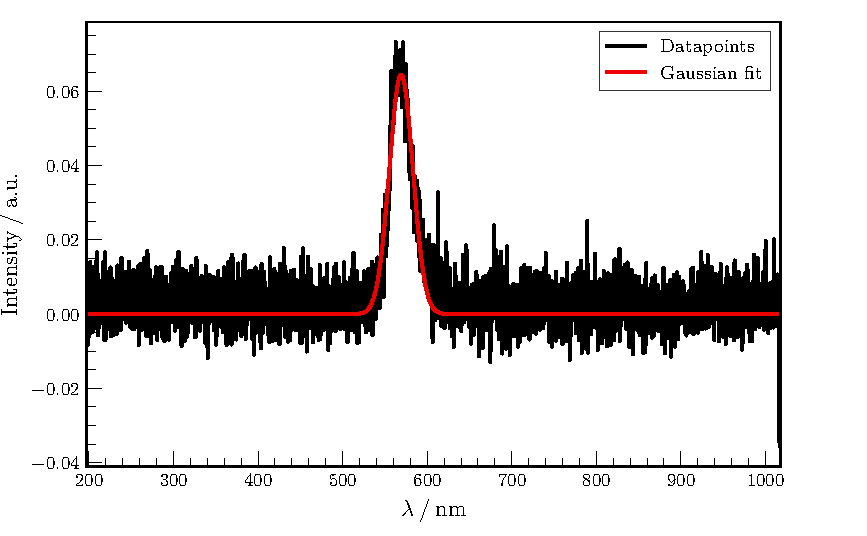
\includegraphics[width=\textwidth]{plots/LED-Green.pdf}
%     \caption{Green LED lightsourse}
%     \label{fig:LEDG}
% \end{subfigure}
% \begin{subfigure}{.3\textwidth}
%     \centering
%     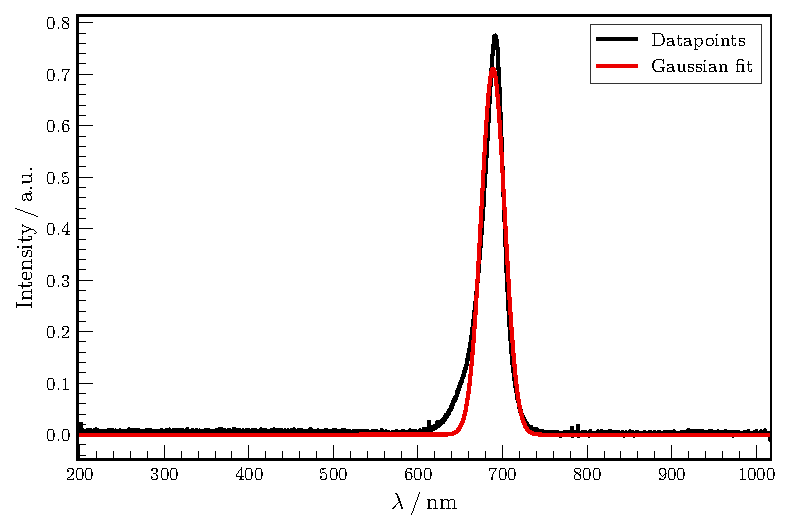
\includegraphics[width=\textwidth]{plots/LED-Red.pdf}
%     \caption{Red LED lightsourse}
%     \label{fig:LEDR}
% \end{subfigure}
% \begin{subfigure}{.3\textwidth}
%     \centering
%     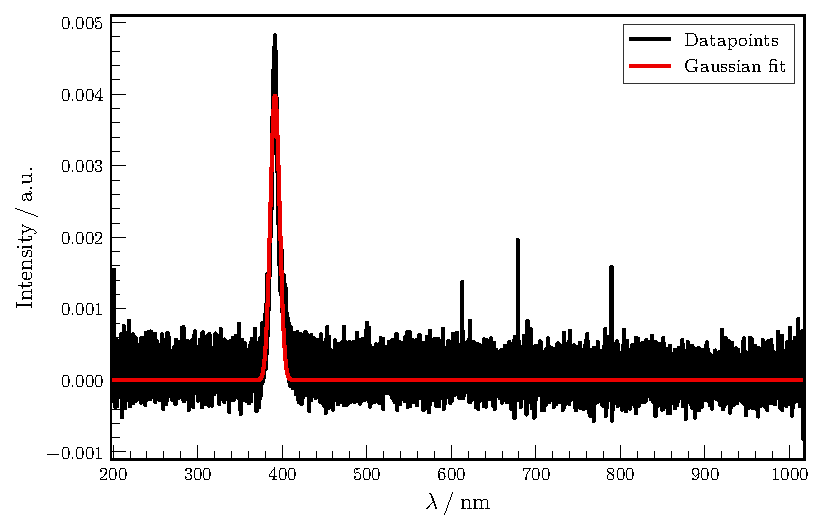
\includegraphics[width=\textwidth]{plots/LED-UV.pdf}
%   \caption{UV LED lightsourse}
%     \label{fig:LEDUV}
% \end{subfigure}
% \caption{Spectral measurement of different LED lightsourse. A Gaussian fit is implemented around the emmision peak.}
% \end{figure*}

%%one figure inside the collums
% \begin{figure}
%     \captionsetup{width=0.9\linewidth}
%     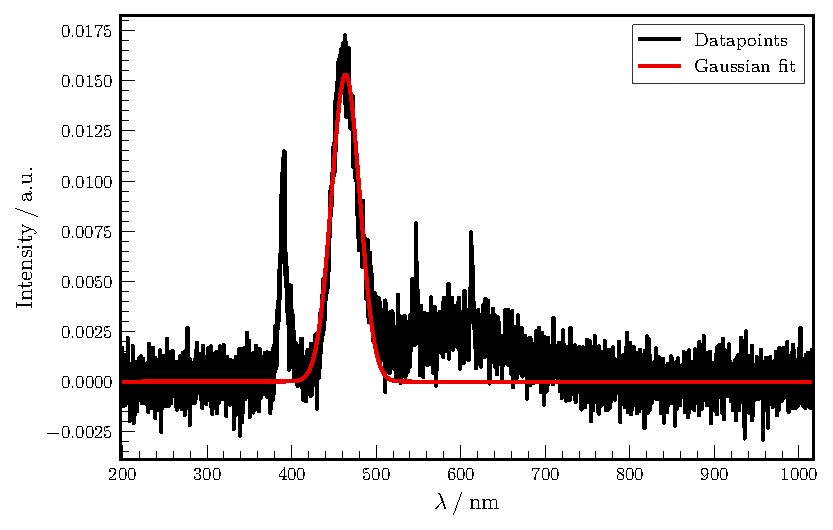
\includegraphics[width=0.5\textwidth]{plots/Samp_A_D.pdf}
%   \caption{Spectral measurement of sample A, excited by a UV-LED lightsource. A Gaussian fit of the peak contributed by luminescense is implemented.}
%     \label{fig:Samp_A_D}
% \end{figure}

\section{Results}
\label{sec:Results}

All characterization steps are done for both samples, where sample A is produced by a perovskite deposited with a slowly evaporated dissolvant 
and sample B with a fast crystallization of the active perovskite layer by introducing an antisolvant.

\subsection{Optic analyzis}
\label{sec:optic-analyzis}

\begin{figure*}
    \centering
\begin{subfigure}{.4\textwidth}
    \centering
    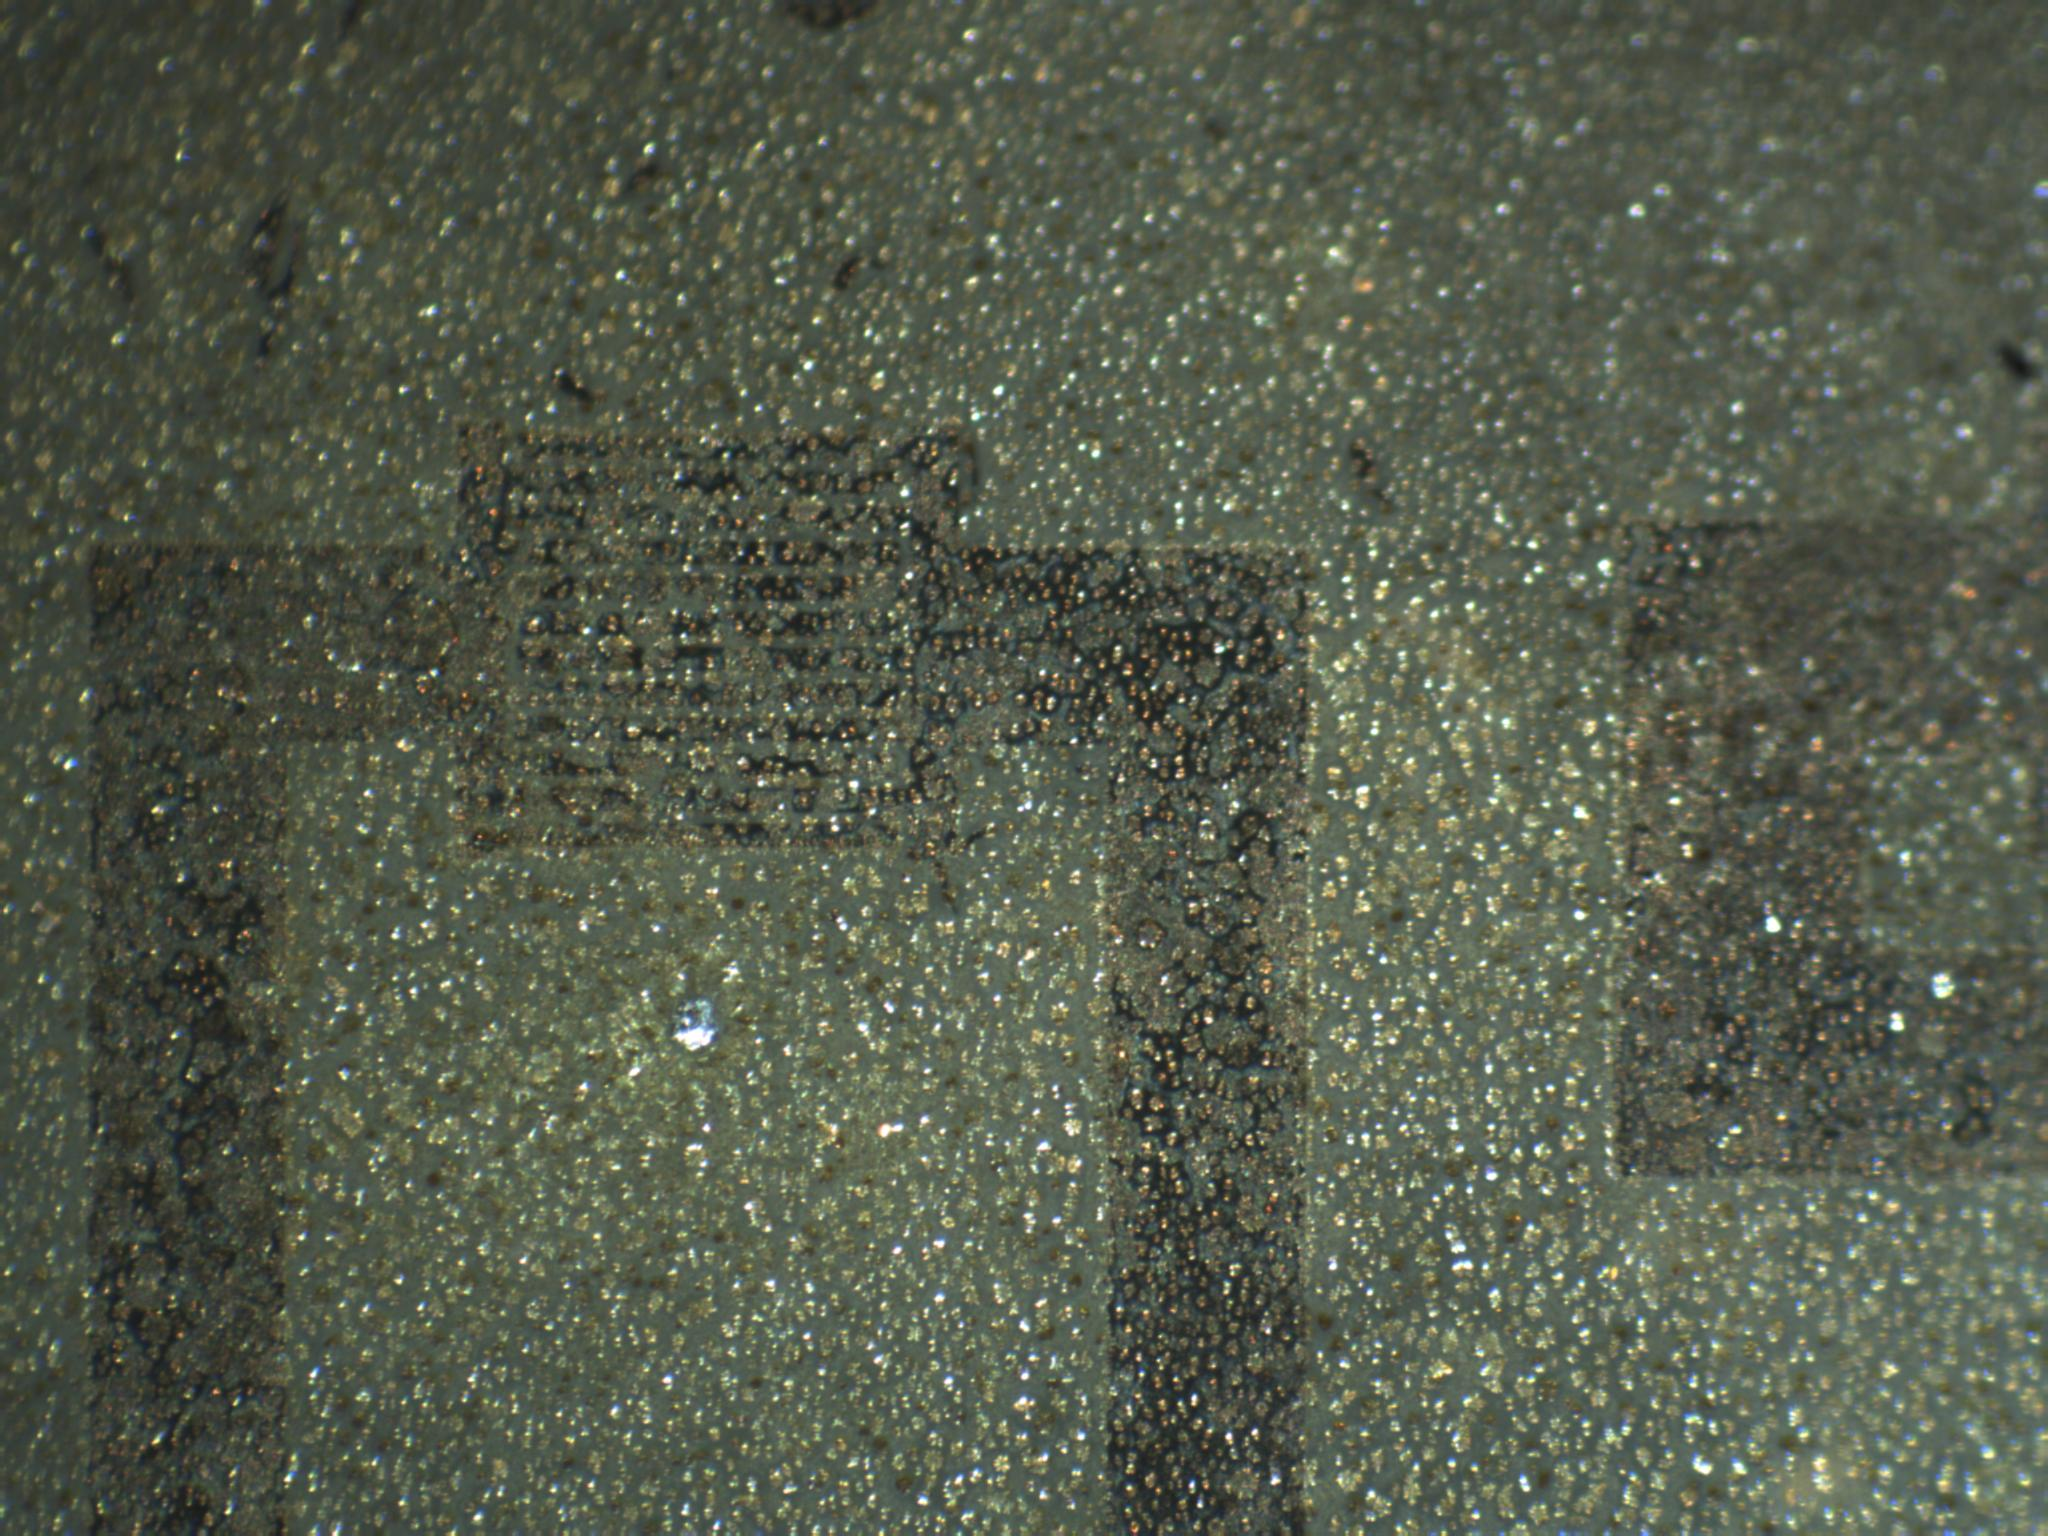
\includegraphics[width=\textwidth]{Data/SampleA_2xzoom.jpg}
    \caption{Front lightning}
\end{subfigure}
\begin{subfigure}{.4\textwidth}
    \centering
    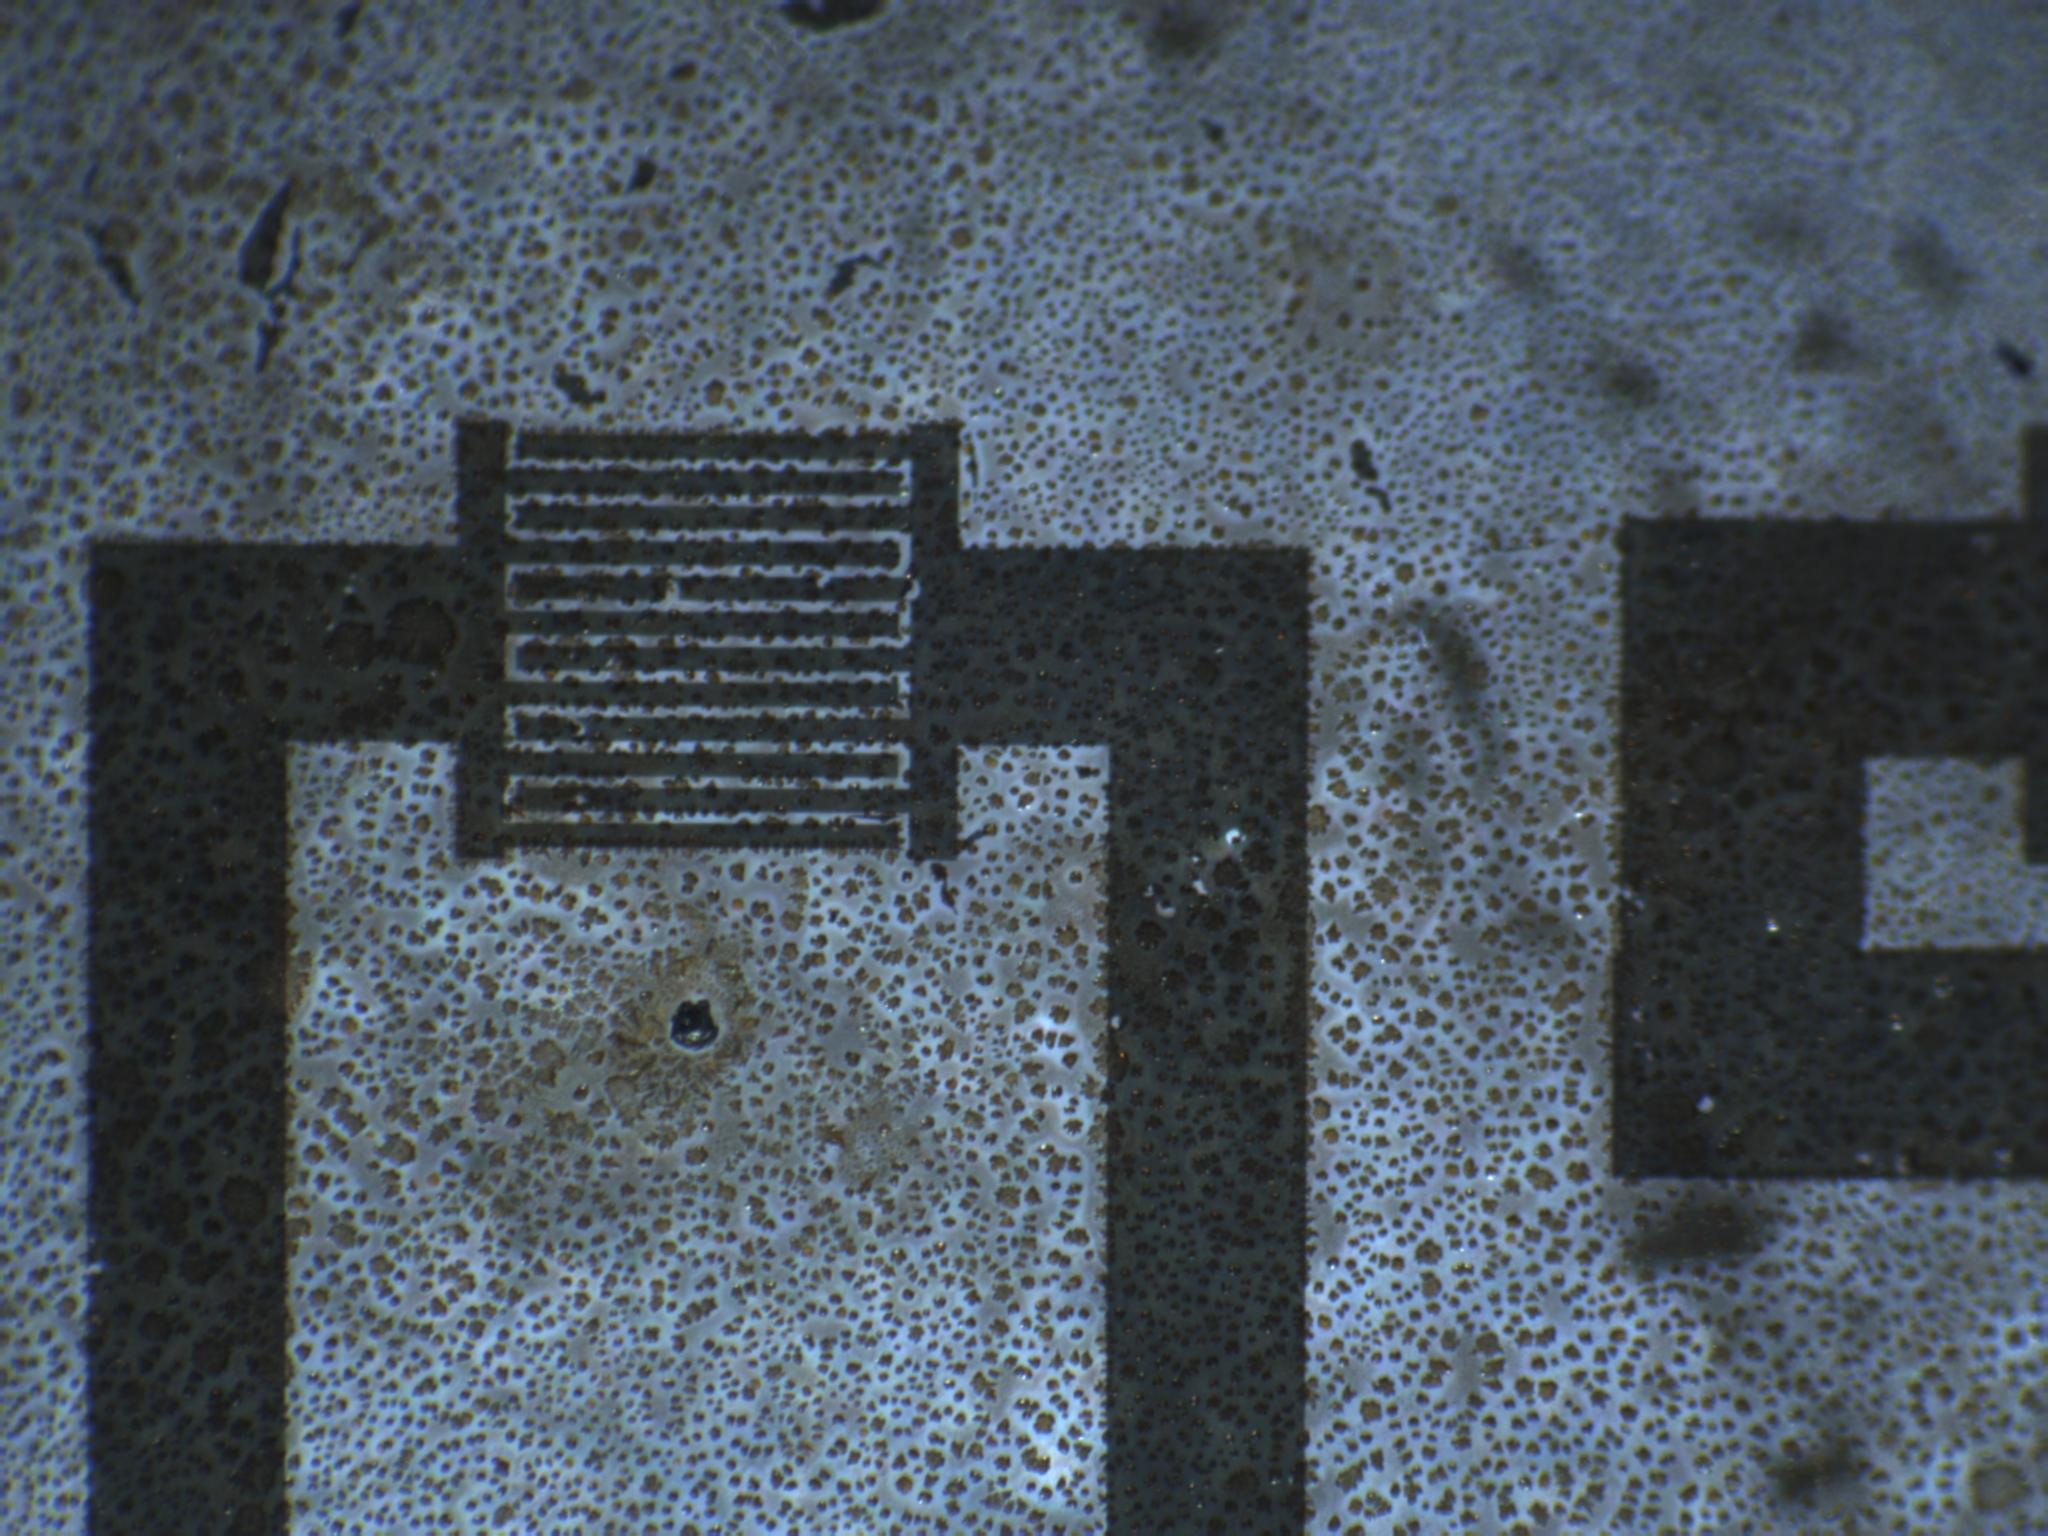
\includegraphics[width=\textwidth]{Data/SampleA_x2zoom_transmission.jpg}
    \caption{Background transmission lightning}
\end{subfigure}
\caption{Microscopic photography with x2 zoom, of no-antisolvant sample A.}\label{fig:optic-A}
\end{figure*}


\begin{figure*}
    \centering
\begin{subfigure}{.4\textwidth}
    \centering
    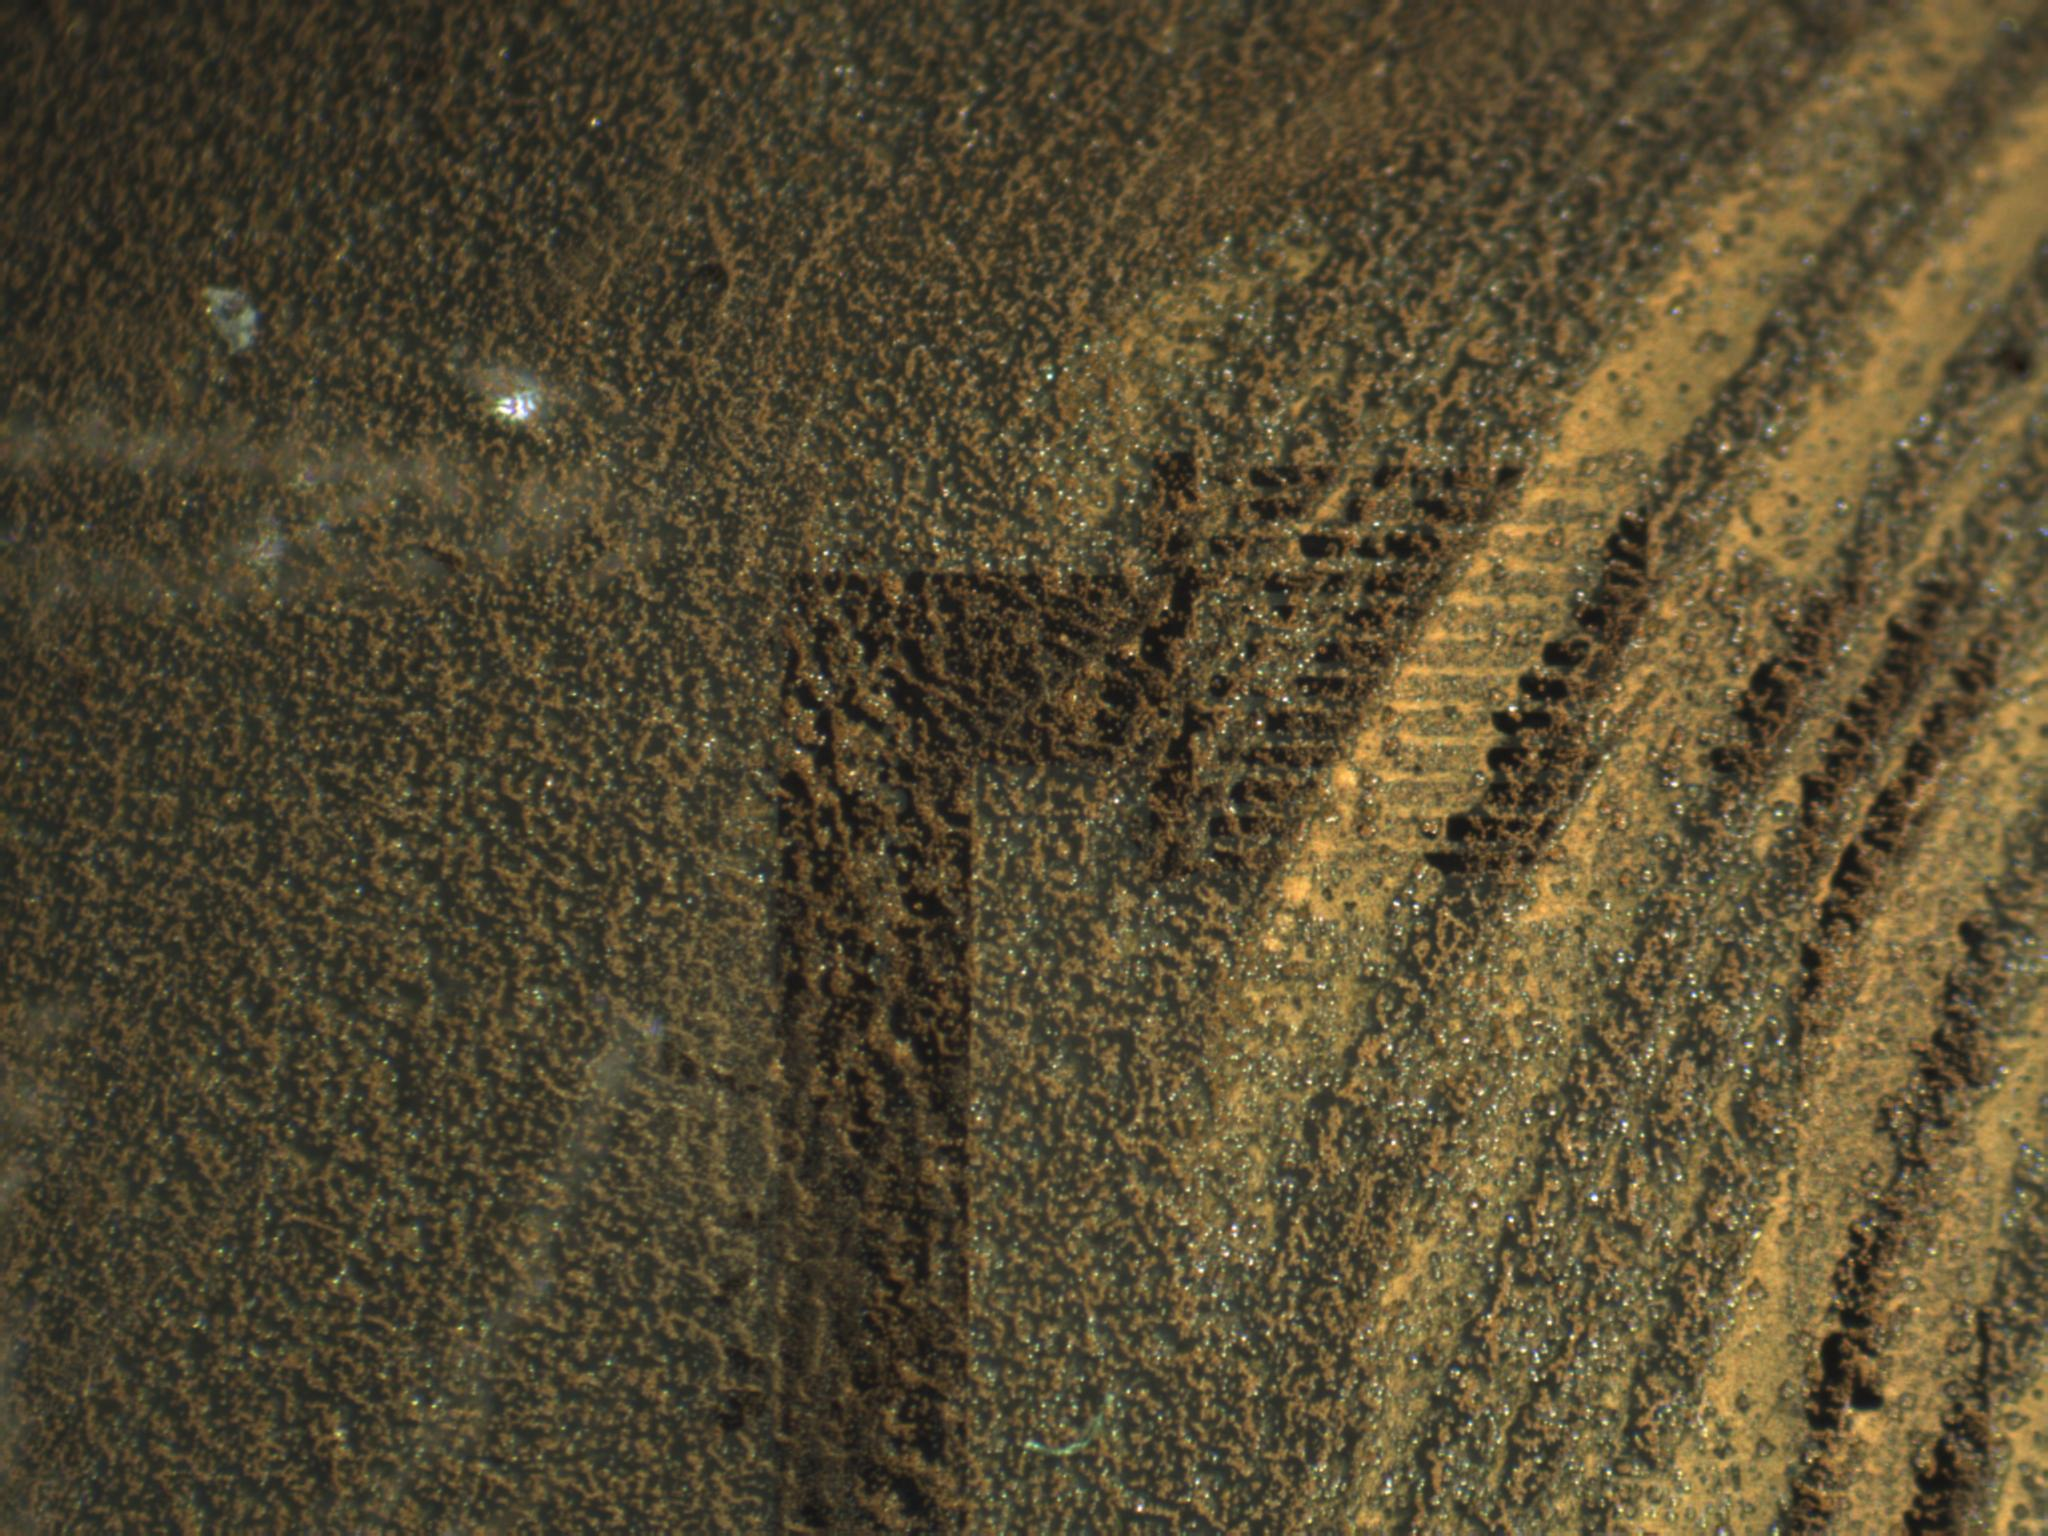
\includegraphics[width=\textwidth]{Data/SampleB_2xzoom.jpg}
    \caption{Front lightning}
\end{subfigure}
\begin{subfigure}{.4\textwidth}
    \centering
    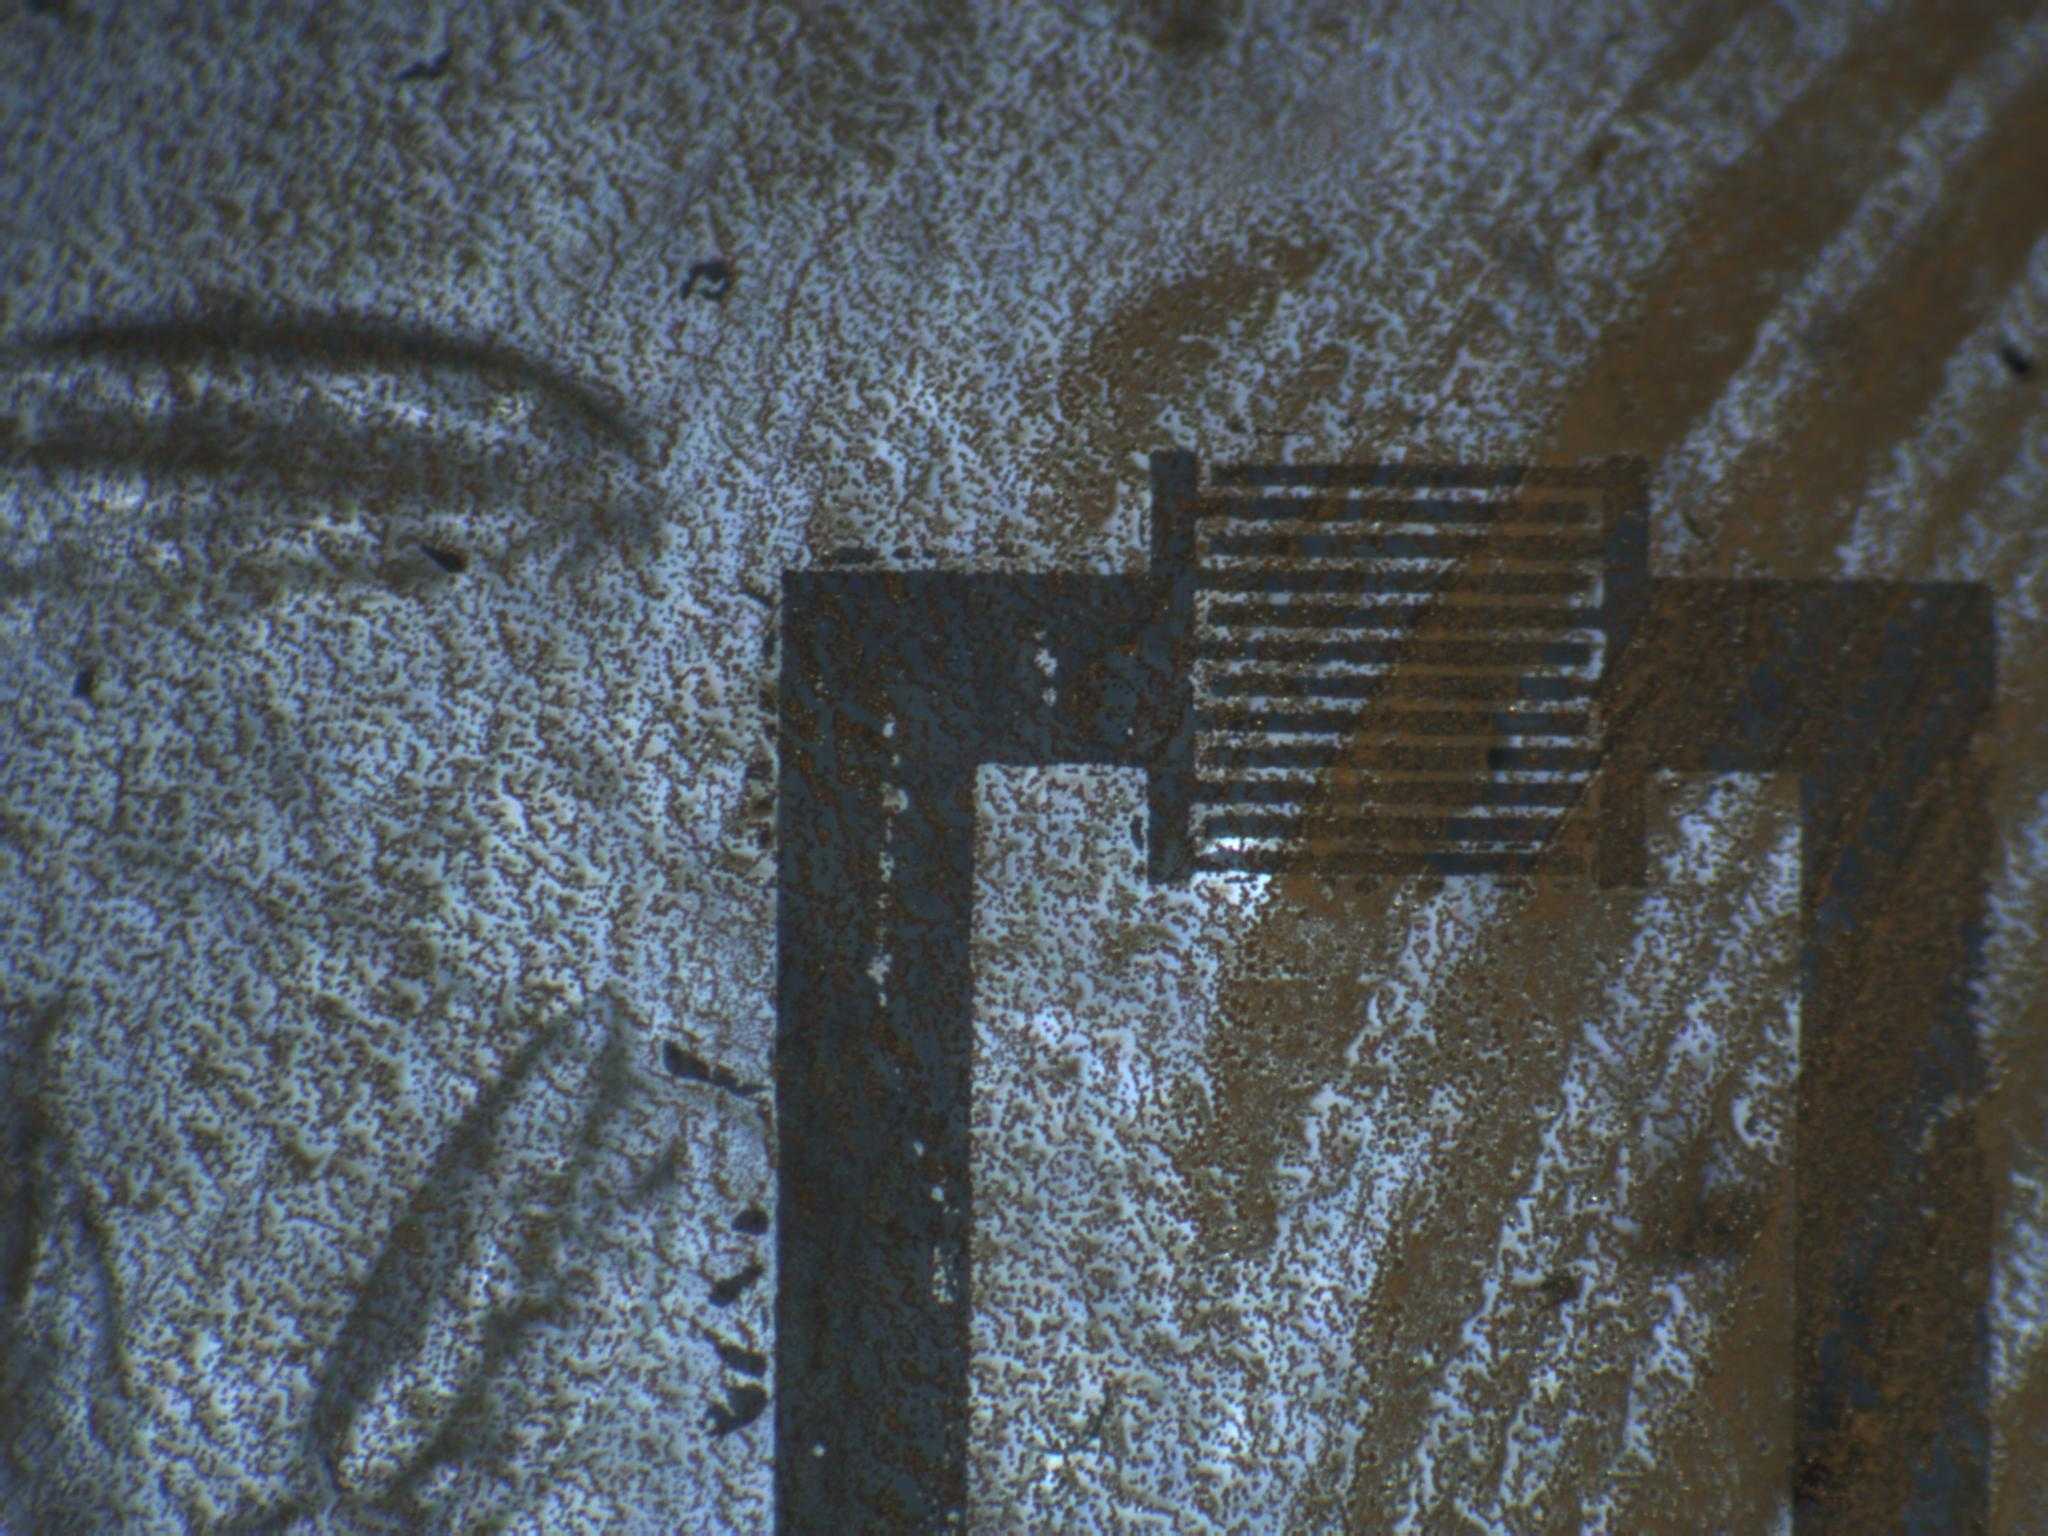
\includegraphics[width=\textwidth]{Data/SampleB_x2zoom_transmission.jpg}
    \caption{Background transmission lightning}
\end{subfigure}
\caption{Microscopic photography with x2 zoom, of antisolvant sample B.}\label{fig:optic-B}
\end{figure*}

In all pictures the contacts seem to be well shaped, so one can expect a functioning electronic connection.
Comparing the figures \ref{fig:optic-A} and \ref{fig:optic-B}, one can see that the reflecting crystals on the surface appear much smaller, almost like a kind of mud on the sample B.
Also the color intensity is stronger for sample B.

\subsection{Electronic analyzis}
\label{sec:elec-analyzis}

\begin{figure*}
    \centering
\begin{subfigure}{.4\textwidth}
    \centering
    \includegraphics[width=\textwidth]{plots/A_dark.pdf}
    \caption{dark}
\end{subfigure}
\begin{subfigure}{.4\textwidth}
    \centering
    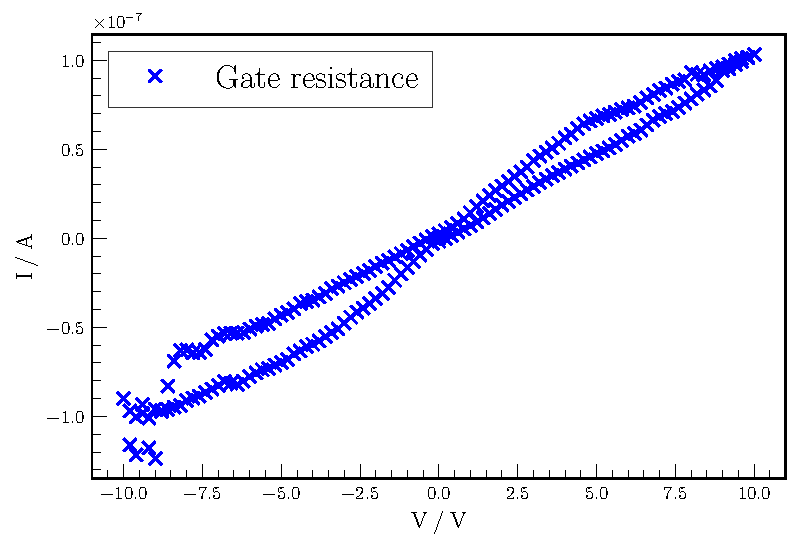
\includegraphics[width=\textwidth]{plots/A_light.pdf}
    \caption{illuminated}
\end{subfigure}
\caption{Gate hysterisis in a V-I plot of the sample A in dark and luminated conditions.}\label{fig:hyst-A}
\end{figure*}


\begin{figure*}
    \centering
\begin{subfigure}{.4\textwidth}
    \centering
    \includegraphics[width=\textwidth]{plots/B_dark.pdf}
    \caption{dark}
\end{subfigure}
\begin{subfigure}{.4\textwidth}
    \centering
    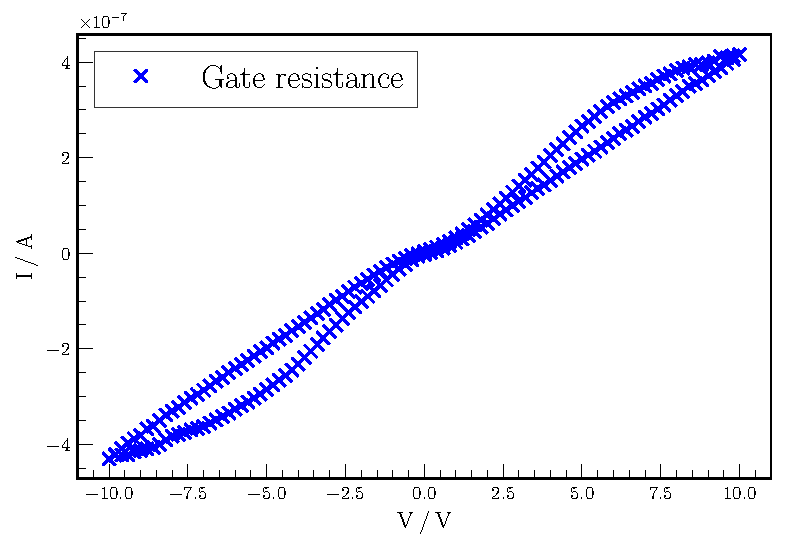
\includegraphics[width=\textwidth]{plots/B_light.pdf}
    \caption{illuminated}
\end{subfigure}
\caption{Gate hysterisis in a V-I plot of the sample B in dark and luminated conditions.}\label{fig:hyst-B}
\end{figure*}

For both samples, one can see a hysteresis of the gate circuit in figure \ref{fig:hyst-A} and \ref{fig:hyst-B}.
Further, the slope which is proportional to the conductivity increases, when the sample is luminated. 
In other words, the resistance of the sample decreases as the sample is illuminated, so both of the samples are sufficient to be used as a linear photodetector, combined with a resistivity measurement aparatus.
 
Refering figure \ref{fig:dynamic}, which shows the time dependent gate current while the light exposion is changed from dark to bright every 5 seconds, shows clearly a current change.
Therefore, it is shown, that the sample circuit can be used as a on/off photodetector.

\begin{figure}
    \captionsetup{width=0.9\linewidth}
    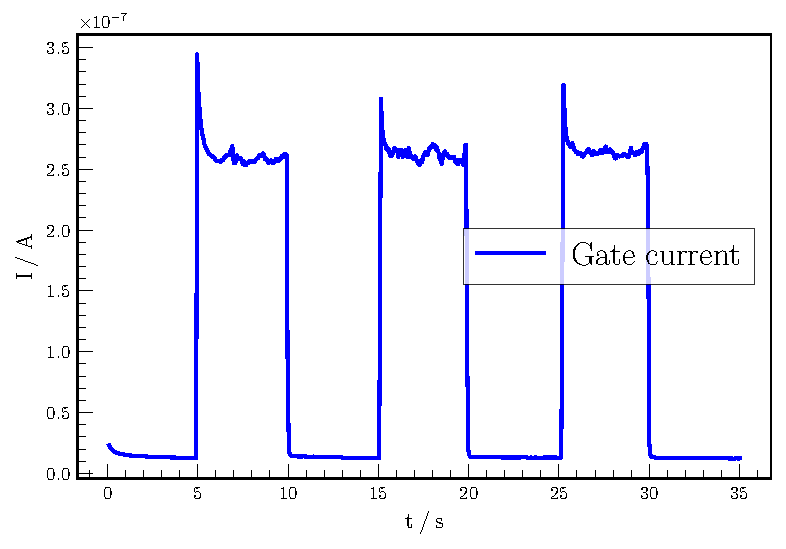
\includegraphics[width=0.5\textwidth]{plots/dynamic.pdf}
  \caption{Gate current of sample B, whiile the illumination is turned on and off every $\SI{5}{\s}$.}
    \label{fig:dynamic}
\end{figure}

% luminated = steigung I/U größer = conductance größer = widerstand kleiner